% Self-contained: paste into Overleaf as main.tex and select pdfLaTeX.
% The complete report, including references, is two pages.
% Graphs use the repository's frozen test results; no image uploads are needed.
\documentclass[10pt,a4paper,twocolumn]{article}
\usepackage[margin=0.62in]{geometry}
\usepackage[T1]{fontenc}
\usepackage{lmodern,microtype}
\usepackage{amsmath,amssymb,booktabs}
\usepackage{xcolor,pgfplots,caption,titlesec}
\usepackage[hidelinks]{hyperref}
\pgfplotsset{compat=1.18}
\definecolor{routeblue}{HTML}{3E51D4}
\definecolor{routegray}{HTML}{8A95A8}
\definecolor{routeamber}{HTML}{C18B2D}
\definecolor{routeteal}{HTML}{16836F}
\setlength{\columnsep}{0.23in}
\setlength{\parindent}{0.9em}
\setlength{\parskip}{0pt}
\setlength{\textfloatsep}{8pt}
\setlength{\floatsep}{6pt}
\setcounter{topnumber}{1}
\setlength{\abovedisplayskip}{5pt}
\setlength{\belowdisplayskip}{5pt}
\titlespacing*{\section}{0pt}{7pt}{3pt}
\titleformat{\section}{\normalsize\bfseries}{\thesection.}{0.4em}{}
\captionsetup{font=small,labelfont=bf,skip=4pt}
\pagestyle{plain}
\raggedbottom
\newcommand{\ind}{\mathbf{1}}

\begin{document}
\twocolumn[{
\begin{center}
  {\small\textbf{GitHub:}
  \url{https://github.com/1amKhush/freshroute-rl}}\\[3pt]
  {\small\textbf{Team:} Khushvendra Singh (B24CM1075)
  \quad Aditya Ranjan (B24CM1004)}\\[7pt]
  {\LARGE\bfseries FreshRoute RL}\\[3pt]
  {\large Staleness-Aware Read Routing for Distributed Databases}\\[5pt]
  {\small AI Assignment 2: Reinforcement Learning Mini Project}
\end{center}
\vspace{4pt}
}]

\noindent\textbf{Abstract.}
FreshRoute RL learns which database replica should answer each read across
different geographic regions. A simulator with fixed random seeds models how
routing affects queues and asynchronous replication over time. A Deep
Q-Network (DQN) balances response time, data freshness, and read failures.
Tests on unseen random seeds compare learned routing with fixed rules. An
interactive laboratory shows the observations, action values, and outcomes
behind each decision.

\section{Practical problem and objective}
Reading from the nearest replica can return stale data. Sending every read to
the write leader can overload its queue. The system has replicas in Mumbai,
Frankfurt (the leader), and Virginia. Each request specifies a client region,
an allowed timestamp lag $b_t$, and a response deadline $d_t$. The goal is to
learn a routing policy that maximizes expected discounted reward,
\[
 J(\pi)=\mathbb{E}_{\pi}\!\left[\sum_{t\geq0}\gamma^t r_t\right],
 \qquad \gamma=0.95.
\]
Each choice changes later queue lengths and how followers apply writes, making
this a sequential control problem. Both agents learn by interacting with the
environment. Fixed routing rules are used only for comparison.

\section{Reinforcement learning formulation}
\textbf{State space $\mathcal{S}$.}
The agent receives a bounded observation
$s_t\in\mathcal{S}\subseteq[0,1]^{26}$:
three client-region and three request-class one-hot entries,
$b_t/500$, $d_t/240$, and six features for each of three replicas. For replica
$i$, these are
\[
\begin{aligned}
 \phi_{i,t}=\bigl(&u_{i,t},\ \mathrm{RTT}_{i,t}/250,
          \ q_{i,t}/(q_{i,t}+100),\\
       &\tau_{i,t}/(\tau_{i,t}+200),\ v_{i,t}/(v_{i,t}+10),\\
       &\delta_{i,t}/(\delta_{i,t}+200)\bigr),
\end{aligned}
\]
where $u$ is online status, $q$ is queued work, $\tau$ is timestamp lag,
$v$ counts committed versions not yet applied, and $\delta$ is replication
delay. Times are in milliseconds. Thus $3+3+2+3(6)=26$.
Freshness is measured as
$\tau_{i,t}=T_{\mathrm{latest},t}-T_{\mathrm{applied}(i),t}$,
using commit timestamps. A replica that has applied all writes has zero lag,
even if no write is recent. Write histories and workload phase are hidden, so
this summary is not guaranteed to be a complete Markov state.

\textbf{Action space $\mathcal{A}$.}
The discrete space is $\{0,1,2\}$: read from Mumbai, Frankfurt, or Virginia,
respectively. An offline replica can still be chosen, so the agent must learn
the resulting failure cost. Retries and quorum reads are not available.

\newpage % Start the reward definition at the top of the second column.

\textbf{Reward function $R$.}
For $i=a_t$, latency is computed as
$\widehat{\ell}_t=\mathrm{RTT}_{i,t}+q_{i,t}+w_i$, where
$(w_0,w_1,w_2)=(14,22,14)$ ms. The failure flag and recorded latency are
\[
 f_t=\ind\{u_{i,t}=0\ \text{or}\ \widehat{\ell}_t>d_t\},\qquad
 \ell_t=(1-f_t)\widehat{\ell}_t+f_t d_t.
\]
With $[x]_+=\max(x,0)$, the implemented reward is
\[
\boxed{\displaystyle
 r_t=-\frac{\ell_t}{d_t}
 -2(1-f_t)\min\!\left(\frac{[\tau_{i,t}-b_t]_+}{\max(b_t,50)},2\right)
 -4f_t.}
\]
Dividing latency by the deadline makes costs comparable across requests.
Staleness beyond the budget gets a capped penalty; the 50 ms floor handles
zero-budget requests. Failures receive reward $-5$ and no freshness credit.
Joint service-level agreement (SLA) success is
$\ind\{f_t=0,\tau_{i,t}\leq b_t\}$: the reward encourages freshness but does
not enforce a hard consistency constraint.

\section{Environment and learning algorithm}
The custom Gymnasium simulator advances by 12 ms per request. Each read adds
service work to the chosen online replica, even if the read times out. Online
replicas drain their queues and receive background work; follower replication
delay also depends on queue pressure. Writes, asynchronous version replay,
failures, and workload changes produce the next observation. Episodes truncate
after 160 reads; learning still bootstraps future value at this time limit.
Reads use snapshots taken at dispatch, with these request classes:
\begin{center}
\small
\begin{tabular}{lrr}
\toprule
Class & Lag budget $b_t$ (ms) & Deadline $d_t$ (ms)\\
\midrule
Latest  & 0   & 240\\
Bounded & 100 & 180\\
Relaxed & 500 & 140\\
\bottomrule
\end{tabular}
\end{center}

The main agent is vanilla DQN~\cite{dqn,sb3}: a
$26\!\rightarrow\!128\!\rightarrow\!128\!\rightarrow\!3$ network with
experience replay and a target network. It learns by minimizing Huber error
against the one-step target
\[
 y_t=r_t+\gamma(1-z_t)\max_{a'}Q_{\theta^-}(s_{t+1},a'),
\]
where $z_t$ marks true termination, not the episode time limit.
Learning rate is $10^{-4}$, replay capacity $100{,}000$, batch size 64, target
update interval 1,000 steps, and one gradient update follows every four
interactions after a 5,000-step warm-up. Exploration decreases from
$\epsilon=1$ to $0.05$ over the first 70\% of training; evaluation uses
$\arg\max_a Q_{\theta}(s,a)$. DQN handles real-valued telemetry without
listing every possible state combination.

A separate tabular Q-learning agent~\cite{qlearning} groups region,
request class, availability, queue, and freshness into coarse buckets, with
$\alpha=0.12$, $\gamma=0.95$, and 192,000 demonstration interactions. It is
not included as a paired baseline in the final DQN tests.

\clearpage % Page 2: experiments, graphs, interface, and references.
\section{Experimental protocol and results}
Training includes balanced traffic, write bursts, regional outages, and shifts
in client traffic. Five full-observation DQNs use seeds
7, 23, 47, 71, and 97; each ablation uses 7, 23, and 47. Every model receives 50,000
interactions: 14 models and 700,000 interactions in total. Validation workloads
select checkpoints. A separate 30-seed validation matrix selects demonstration
seed 71 using mean reward with equal weight for all four workloads. The
selection and model hashes are fixed before testing.

Final testing~\cite{evidence} uses seeds 200000--200029 in each regime, with 160 requests per
episode. Policies receive the same external workload draws, while their own
queues evolve separately. Controls are \emph{nearest}, \emph{leader-only}, and
uniform \emph{random}; none provides training labels or a hidden routing
fallback.

\begin{figure}[t]
\centering
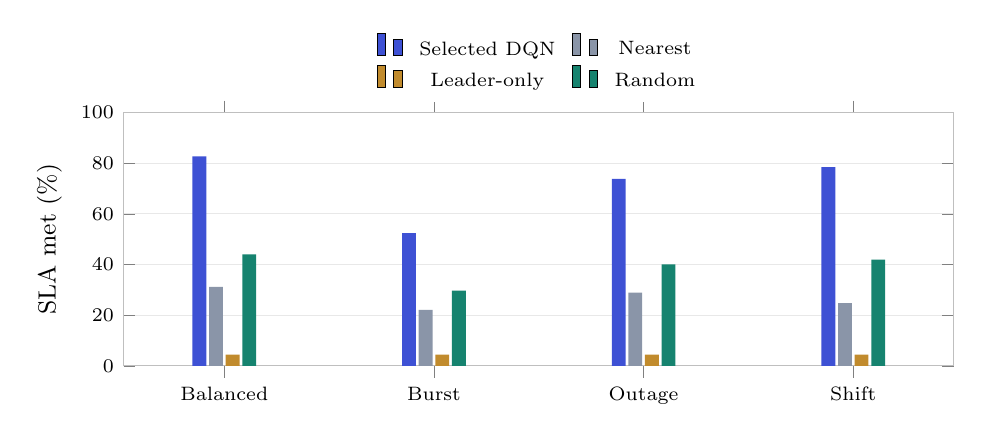
\begin{tikzpicture}
\begin{axis}[
  width=\columnwidth,height=4.8cm,
  ybar=1pt,bar width=5pt,
  ymin=0,ymax=100,ytick={0,20,40,60,80,100},
  ylabel={SLA met (\%)},
  symbolic x coords={Balanced,Burst,Outage,Shift},xtick=data,
  enlarge x limits=0.16,
  tick label style={font=\scriptsize},label style={font=\small},
  ymajorgrids=true,grid style={gray!18},axis line style={gray!50},
  legend style={font=\scriptsize,at={(0.5,1.04)},anchor=south,
    legend columns=2,draw=none,column sep=4pt},
]
\addplot[fill=routeblue,draw=none] coordinates
  {(Balanced,82.6667) (Burst,52.3333) (Outage,73.7292) (Shift,78.4375)};
\addplot[fill=routegray,draw=none] coordinates
  {(Balanced,31.1875) (Burst,22.0833) (Outage,28.9167) (Shift,24.75)};
\addplot[fill=routeamber,draw=none] coordinates
  {(Balanced,4.4167) (Burst,4.4167) (Outage,4.4167) (Shift,4.4167)};
\addplot[fill=routeteal,draw=none] coordinates
  {(Balanced,44) (Burst,29.6458) (Outage,40) (Shift,41.9167)};
\legend{Selected DQN,Nearest,Leader-only,Random}
\end{axis}
\end{tikzpicture}
\caption{Deadline-and-freshness success on unseen test seeds for the
validation-selected DQN and fixed rules: 30 episodes per workload.}
\label{fig:policies}
\end{figure}

The selected DQN meets both freshness and deadline requirements on 82.7\% of
balanced requests, versus 31.2\% for nearest and 44.0\% for random
(Fig.~\ref{fig:policies}); its mean reward is $-0.763$ and response
availability is 98.8\%. Leader-only meets the SLA on 4.4\% of requests because
sending all reads to the leader overloads its queue at these service rates.
Availability means a data response within the deadline, not replica uptime.

\begin{figure}[t]
\centering
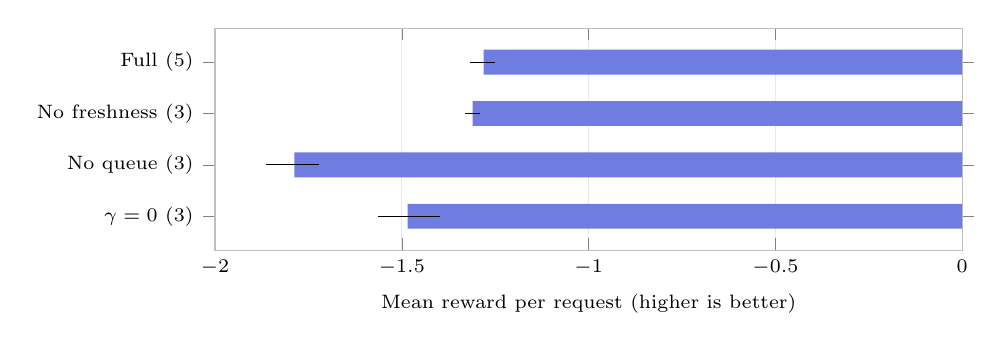
\begin{tikzpicture}
\begin{axis}[
  width=\dimexpr\columnwidth-30pt\relax,height=4.4cm,
  xbar,bar width=9pt,xmin=-2,xmax=0,
  xtick={-2,-1.5,-1,-0.5,0},
  xlabel={Mean reward per request (higher is better)},
  ytick={0,1,2,3},y dir=reverse,
  yticklabels={Full (5),No freshness (3),No queue (3),$\gamma=0$ (3)},
  enlarge y limits=0.22,
  tick label style={font=\scriptsize},label style={font=\scriptsize},
  xmajorgrids=true,grid style={gray!18},axis line style={gray!50},
]
\addplot+[
  fill=routeblue!75,draw=none,
  error bars/.cd,x dir=both,x explicit,
  error bar style={black,thin},error mark options={black},
] table[x=mean,y=id,x error minus=lo,x error plus=hi] {
mean       id lo       hi
-1.281112  0  0.021208 0.016563
-1.310723  1  0.004503 0.005106
-1.787901  2  0.060611 0.052414
-1.484330  3  0.063424 0.072674
};
\end{axis}
\end{tikzpicture}
\caption{Mean test reward with equal weight for all four workloads.
Parentheses count independent training seeds; whiskers show descriptive
95\% percentile bootstrap intervals across those agents.}
\label{fig:ablations}
\end{figure}

Across all five full-agent seeds, macro SLA satisfaction is 71.0\% and mean
reward is $-1.281$. Figure~\ref{fig:ablations} compares separately trained
ablations: no-freshness sets $\tau,v,\delta$ channels to zero; no-queue zeros
$q,\delta$; $\gamma=0$ keeps all observation features. Queue and replication
information help in this setup. The small freshness-ablation gap does not show
that these features are always needed. Discount-ablation differences can also
come from optimization effects. Intervals resample mean results across
training seeds, rather than treating correlated requests as independent.

\newpage % Keep the interface discussion together in the final column.
\section{Interactive system and reproducibility}
A React interface and FastAPI backend show actual observations, the three
learned action values, chosen routes, and measured reward components. Finite
packet animations show fresh, stale, and failed reads, with pause, stepping,
and reduced-motion controls. Live sessions run a frozen policy and let users
inject outages, lag, and load. Eight-step counterfactuals copy the same simulator
and random state to try different first actions without changing the original
session. Q-values are estimates; branch outcomes are measured. The repository
includes runnable code, dependency locks, trained agents, reproduction scripts,
and checksummed traces.

\section{Scope and limitations}
These results come from a synthetic simulator using new seeds within the same
four workloads. They do not establish convergence or production performance.
DQN and tabular Q-learning were not compared on paired final tests. Telemetry
is exact; noisy monitoring, mid-flight failures, leader election, hard
consistency enforcement, and real-database validation remain future work.
Zero timestamp lag alone does not establish linearizability.

% References fit inside the two-page document as well.
\begin{thebibliography}{9}
\small\raggedright
\bibitem{dqn}
V.~Mnih et al., ``Playing Atari with Deep Reinforcement Learning,''
arXiv:1312.5602, 2013.
\url{https://arxiv.org/abs/1312.5602}

\bibitem{sb3}
Stable-Baselines3, ``DQN,'' version 2.9.0 documentation.
\url{https://stable-baselines3.readthedocs.io/en/v2.9.0/modules/dqn.html}

\bibitem{qlearning}
C.~J.~C.~H.~Watkins and P.~Dayan, ``Q-learning,''
\emph{Machine Learning}, vol.~8, pp.~279--292, 1992.
\url{https://www.gatsby.ucl.ac.uk/~dayan/papers/cjch.pdf}

\bibitem{evidence}
K.~Singh and A.~Ranjan, \emph{FreshRoute RL}, source code and frozen
experiment artifacts, 2026. See \texttt{artifacts/releases/evaluation.json},
\texttt{test-matrix.json.gz}, and \texttt{frozen.json}.
\url{https://github.com/1amKhush/freshroute-rl}
\end{thebibliography}
\end{document}
